%! TEX root = /home/simon/Documents/Dagbok_MPPHS_2020-2021/main.tex
\subsection{Måndag 2020-10-26}

Skrev tentan i kommutativ algebra idag. Det gick skitdåligt. Jag lämnade inte in något. Sen byggde jag dator med Kenneth.


\subsection{Tisdag 2020-10-27}

\href{https://github.com/s-n-ushakov/rename-efi-entry}{\color{blue}Här} är ett najjs script för att byta namn på entries i UEFI boot manager.

\subsection{Onsdag 2020-10-28}

Hade integrationsteorimunta idag. Det kändes helt OK även om jag inte kom ihåg allt. Jeff sa att jag var godkännd iaf.

Jag installerade KVM/QEMU för att köra virtuel machines på min dator. Jag kan mounta en .iso \& köra den genom
\begin{verbatim}
qemu-img create -f qcow2 testing_manjaro.img 10G
qemu-system-x86_64 -m 2048 -boot d -enable-kvm -smp 2 -net nic -net user -hda
    testing_manjaro.img -cdrom Downloads/manjaro-xfce-20.1.2-201019-linux58.iso
\end{verbatim}
Jag hittade en najjs \href{https://fosspost.org/use-qemu-test-operating-systems-distributions/}{\color{blue}källa} som förklarade lite om hur man kör QEMU. Den ger en förklaring till ovanstående kommandon:
\begin{figure}[H]
	\centering
	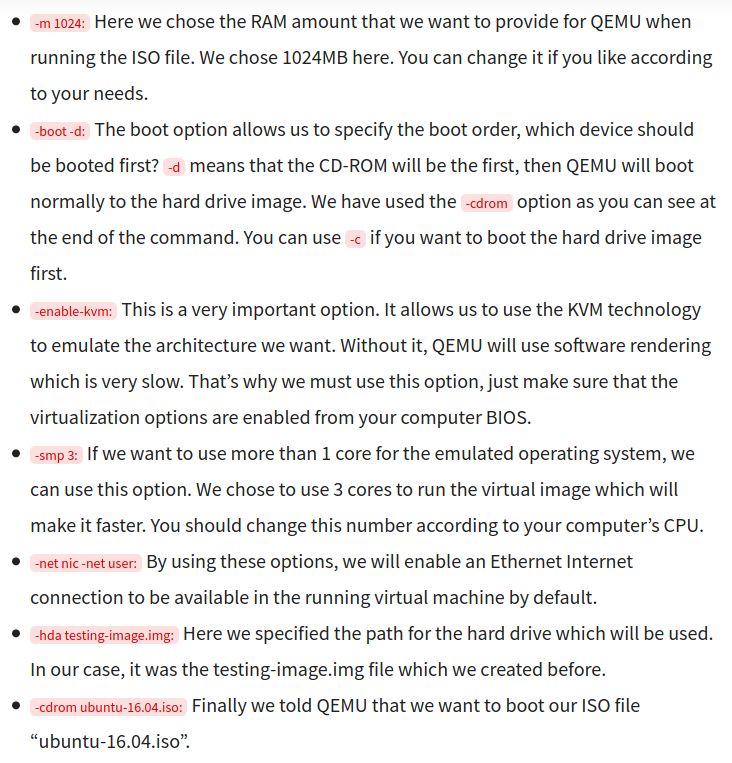
\includegraphics[width=0.8\textwidth]{pics/qemu_explained_example.png}
\end{figure}
Sen efter jag installerat kan jag köra
\begin{verbatim}
qemu-system-x86_64 -m 2048 -boot d -enable-kvm -smp 2 -net nic -net user -hda
    testing_manjaro.img
\end{verbatim}
för att starta det installerade operativsystemet :).


